% !TEX root = ../main.tex

\chapter{绪论}
\section{研究背景和意义}

四旋翼无人机由于其高机动性、易于部署、低成本等优势,在近年来得到了越来越多的商业化应用。例如,航拍无人机已经在电影和媒体行业中得到广泛应用(如图\ref{dji}),消费级航拍无人机的市场也空前繁荣,新奇的航拍视角大幅提高了视觉呈现的吸引力和表现力。无人机集群的灯光表演越来越多地出现在大众的视野中,成为节庆典礼的常客(如图\ref{灯光秀})。在农业领域,植保无人机用于监测作物健康和精准施肥灌溉\cite{tokekar2016agricluture}(如图\ref{植保}),尤其是在地形复杂不利于大型农机作业的地方,显著提高了作物产量和农业资源的使用效率。在自然灾害发生时,四旋翼无人机在紧急搜救和灾后评估中也显示出巨大的潜力\cite{tomic2012}(如图\ref{救援}),它们能够快速进入灾区进行空中勘察,为救援队提供实时数据,有助于优化救援计划并减少救援人员的风险。(以上图片源自网络)

\begin{figure}[htb]
    \centering
    \begin{minipage}[b]{0.49\linewidth}
        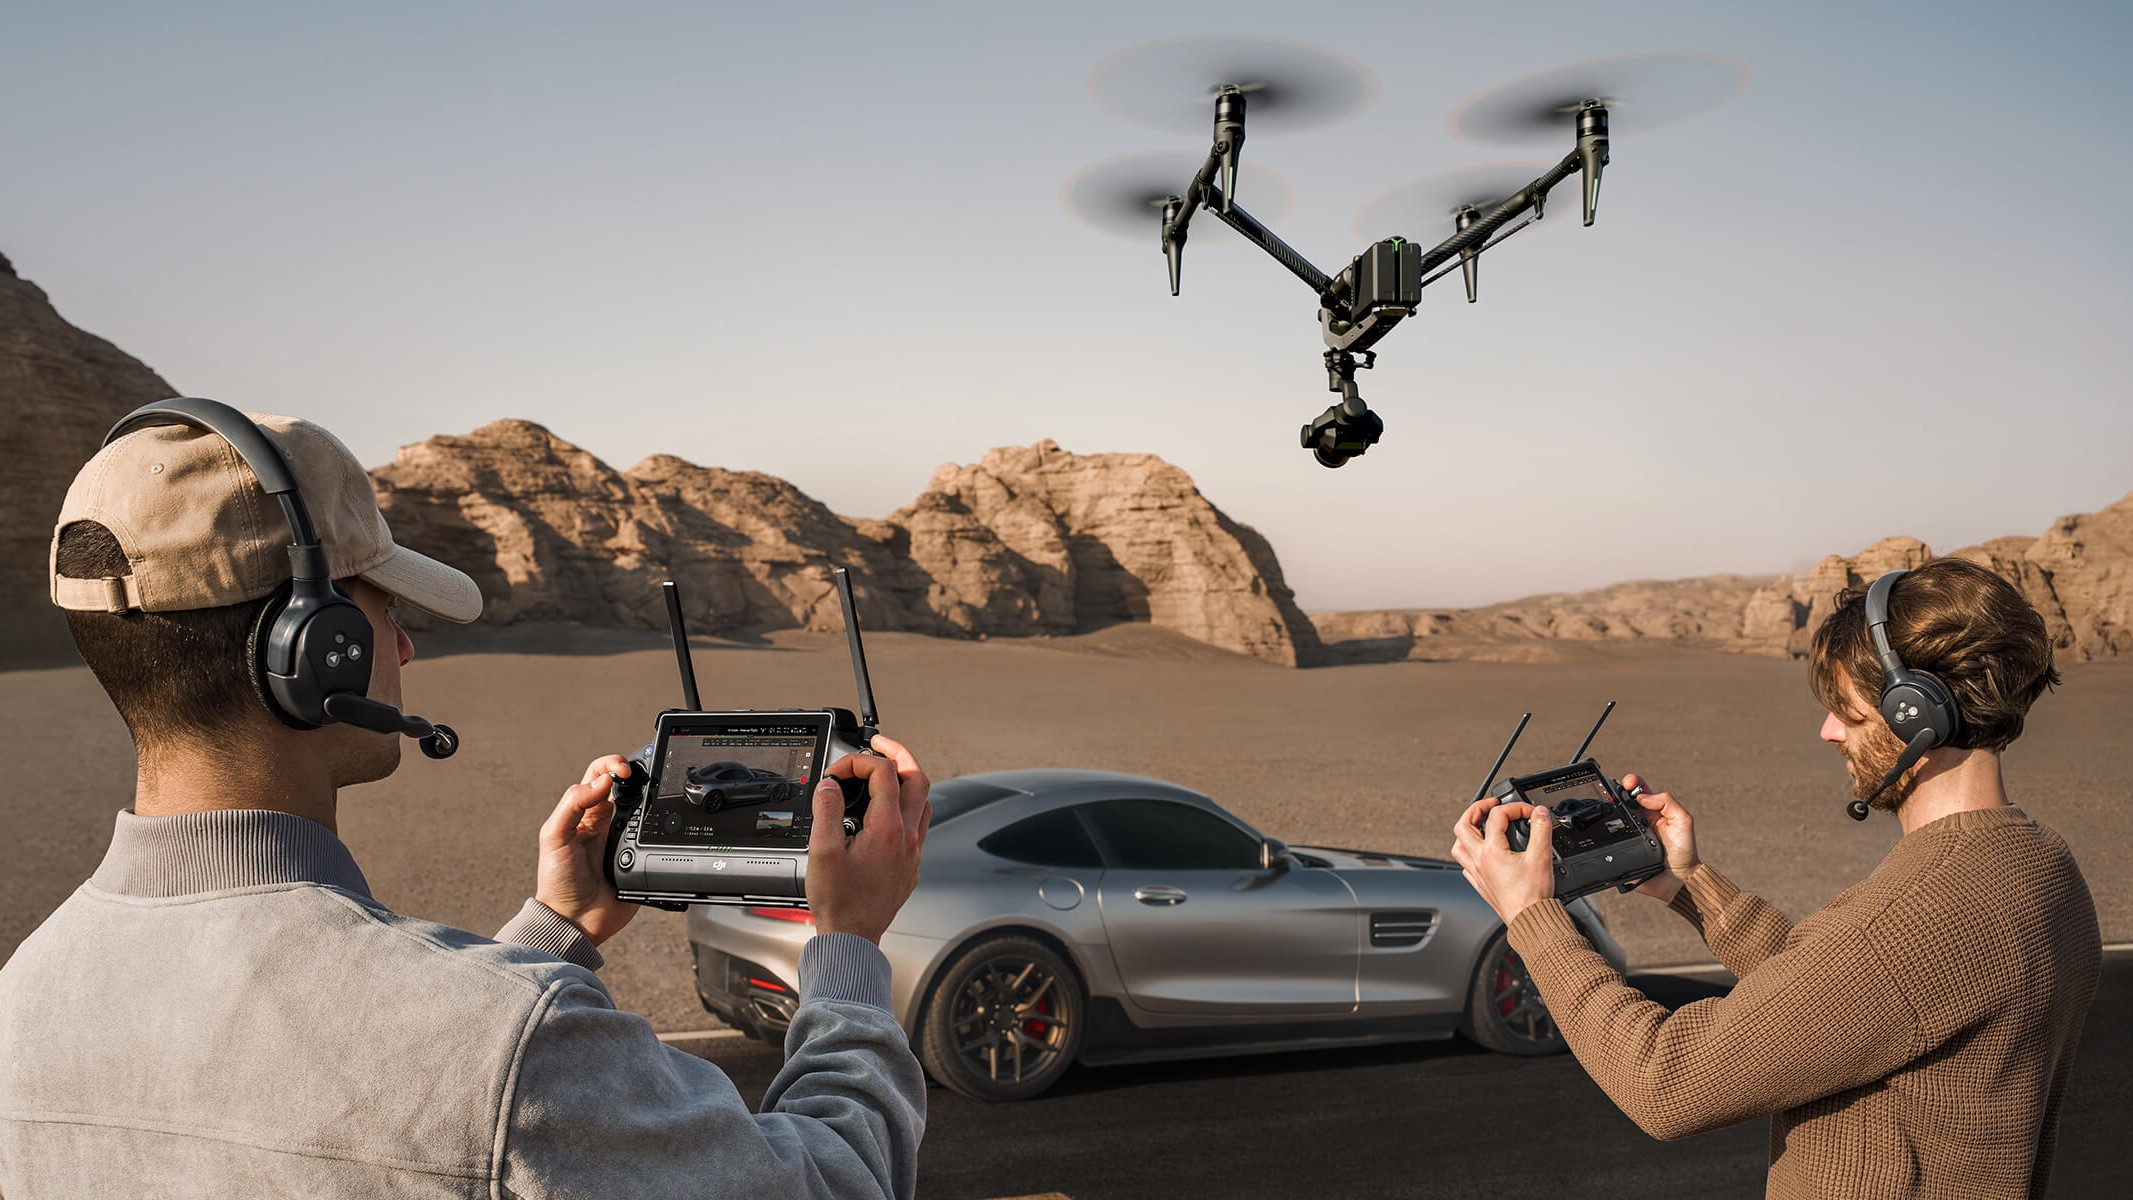
\includegraphics[width=\linewidth]{dji.jpg}
        \caption{航拍无人机拍摄电影}
        \label{dji}
    \end{minipage}
    \hfill % 在图片之间添加一些空间
    \begin{minipage}[b]{0.49\linewidth}
        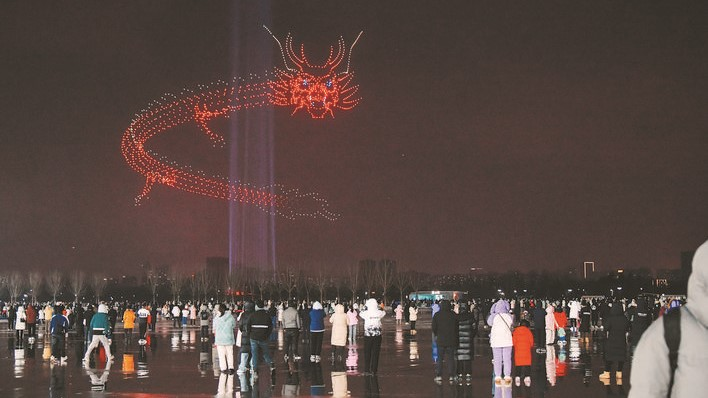
\includegraphics[width=\linewidth]{灯光秀.jpg}
        \caption{无人机集群灯光表演}
        \label{灯光秀}
    \end{minipage}

    %\vspace{1cm} % 在行之间添加一些垂直空间

    \begin{minipage}[b]{0.49\linewidth}
        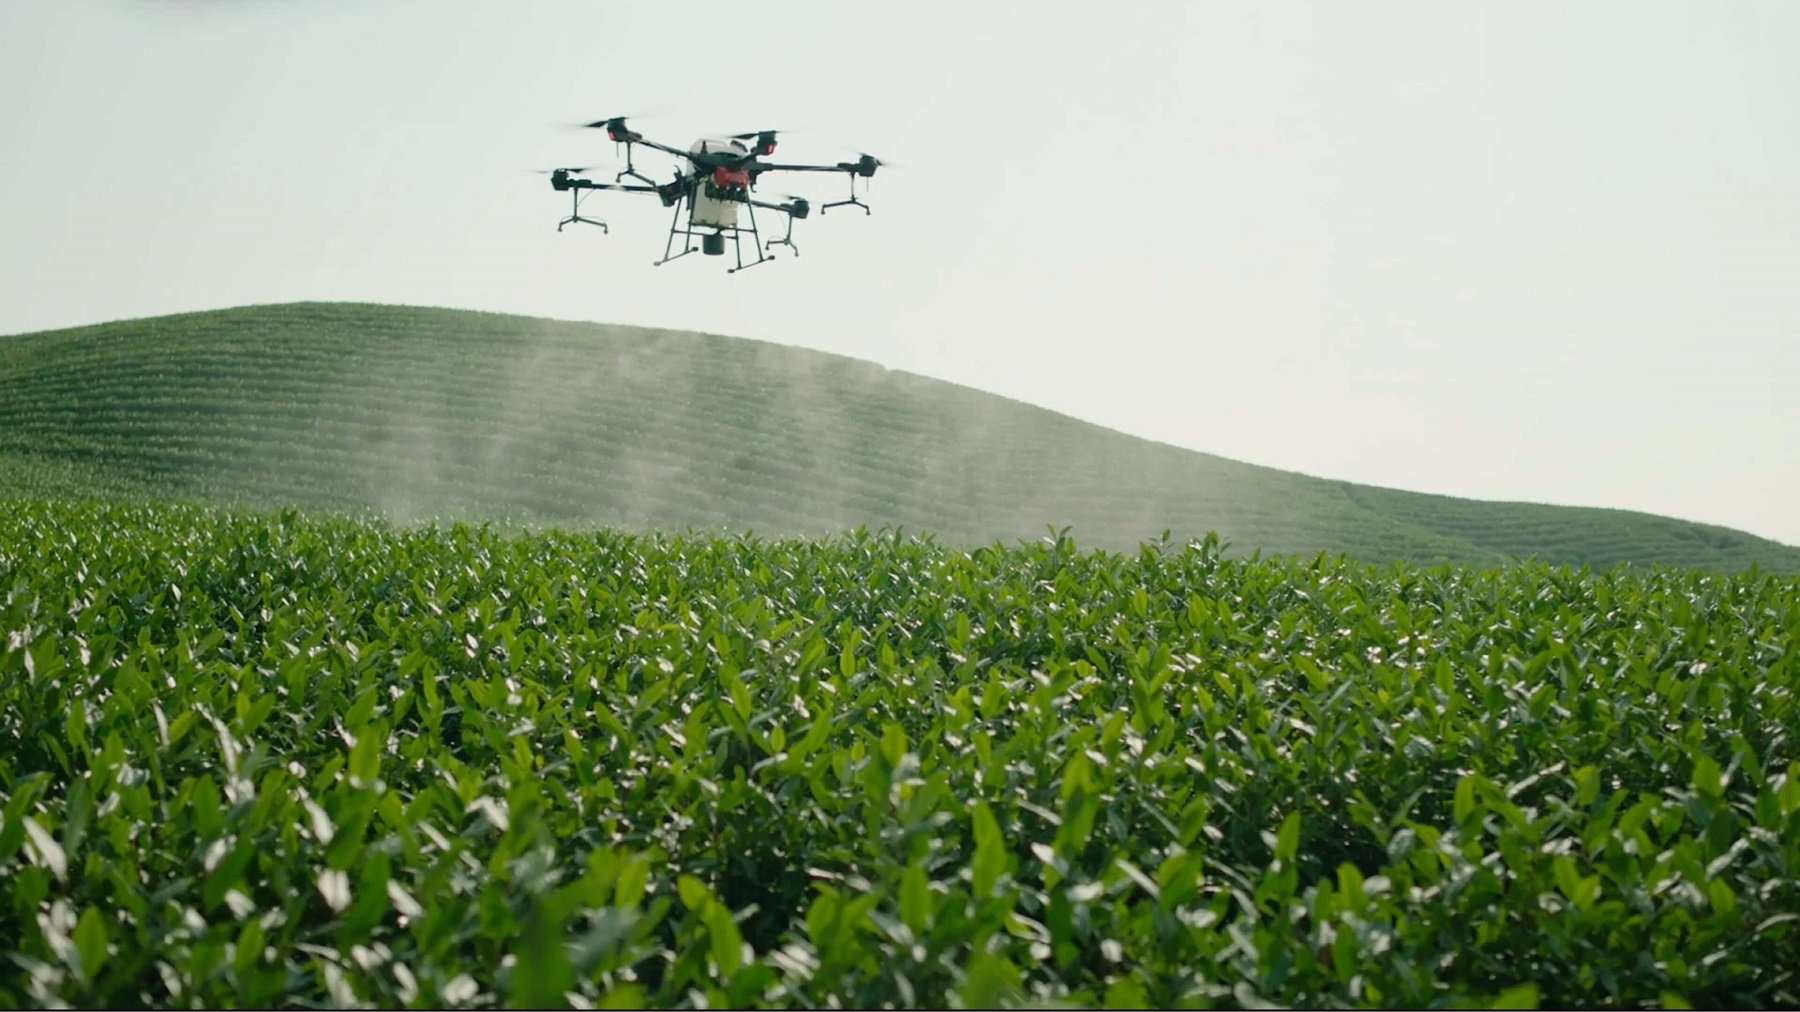
\includegraphics[width=\linewidth]{植保.jpg}
        \caption{植保无人机田间作业}
        \label{植保}
    \end{minipage}
    \hfill
    \begin{minipage}[b]{0.49\linewidth}
        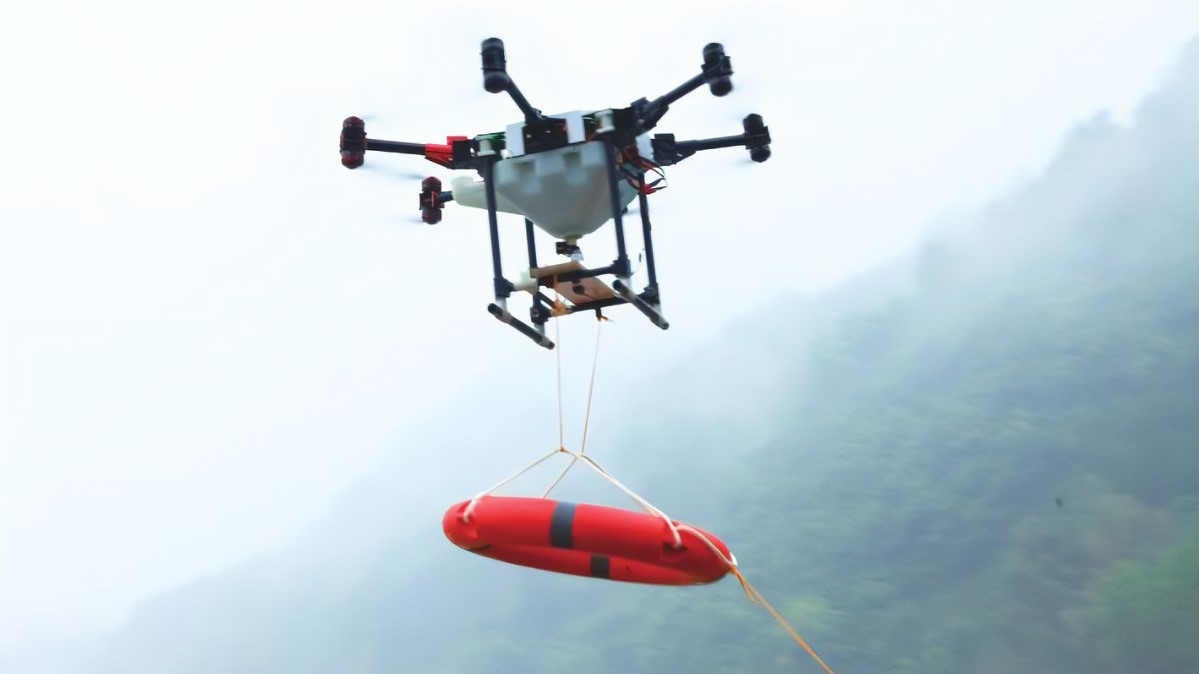
\includegraphics[width=\linewidth]{搜救.jpg}
        \caption{救援无人机水面营救}
        \label{救援}
    \end{minipage}
\end{figure}

尽管四旋翼无人机在许多领域都已经有了落地应用,但它们的运动控制仍然有进步完善的空间。系统的高度非线性、大角度机动时的脆弱稳定性以及传感器对环境噪声的敏感性等仍然是无人机运动控制要面临的技术难题。这些技术难题的存在,限制了无人机在更多高风险或复杂环境中的应用。因此,深入研究和优化四旋翼无人机的运动控制技术,不仅能够推动无人机技术的进一步商业化,还有助于拓宽其在社会服务和经济活动中的应用范围,如更复杂的城市空中交通管理和多无人机协同作业等新兴领域。

综上所述,四旋翼无人机的研究不仅具有重要的技术意义,更在社会经济和安全等多个层面发挥着越来越重要的作用。因此,本研究旨在通过对四旋翼无人机运动控制的深入分析和改进,解决现有的技术难题,为其更广泛的应用奠定坚实的基础。
\section{四旋翼运动控制的研究现状}
四旋翼无人机出于上述的种种优势和应用场景,近年来得到了广泛研究\cite{survey}。四旋翼具有高度机动性的优势,同时也有欠驱动、载荷算力有限和高控制频率的限制。这使得四旋翼成为验证先进控制理论的理想测试平台\cite{La2018}。四旋翼无人机的控制分为两个环路,位置环和姿态环。由于四旋翼输出的推力总是垂直于机身平面向下,因此要控制位置到达设定点,就需要先旋转姿态,以使推力指向设定点。


\begin{figure}[!h]
    \centering
    
\includegraphics[width=0.7\textwidth]{框图.png}
    \caption{四旋翼控制框图}
    \label{框图}
  \end{figure}
  如图\ref{框图},一个典型的四旋翼无人机控制回路会有以下部分组成:
\begin{itemize}
     \item 路径规划,向位置环输入位置设定点
     \item 位置环计算期望推力和期望姿态,将期望姿态发送给姿态环
     \item 姿态环计算期望力矩
     \item 动力分配环节由期望推力和期望力矩计算得到四个电机的控制量
   \end{itemize}
   

随着近年来计算机处理能力的增强以及传感器的发展,关于无人机控制的研究快速发展。
2004年,Samir Bouabdallah将角速度近似等于欧拉角的导数,得到简化后的四旋翼动力学方程,在此基础上他分步解决姿态跟踪和高度跟踪的问题。他使用了简单的闭环反馈作为控制器进行仿真和实机实验,证实了其控制姿态角的能力\cite{boua2007}。但这一阶段的工作还比较粗糙,在姿态角较大时将角速度近似等于欧拉角会带来很大的偏差。其控制器几乎只是依赖调参,抗扰动能力较差,并且也只做到了悬停的高度控制。于是在2005年,Samir Bouabdallah进一步提出了反步法和滑膜控制两种非线性的方法\cite{boua2005},做到了四旋翼的位置控制并增强了抗扰动能力。虽然还是根据近似后的动力学模型,但反步法能够在较高扰动的情况下做到对方向角的控制。而滑膜控制由于开关特性引入了高频低振幅的振动,使得传感器漂移,导致控制效果一般。2007年在此基础上改进的积分反步法\cite{bouabdallah2007full},也就是在将角速度期望设为角度误差的PID,达成了更好的角度控制。但受限于电机的响应速度,抖动仍然存在。积分反步法也应用在了位置控制的环节,做到了自动起降、悬停和避障。这一系列的工作在当年是开创性的,但由于传感器精度和频率、执行器性能的限制,其表现在今天看来还是较为不足。


以上的工作对期望位姿的解算实质上是欠缺物理意义的,而T. Lee于2010年提出了针对四旋翼复杂机动的非线性控制\cite{Lee2010},在没有对动力学近似的情况下,对这个问题做了物理上合理的解答。由于四旋翼的合推力总是垂直于机身平面,所以将位置环通过前馈和反馈控制算出的期望推力方向作为期望的z轴指向,再由用户输入的期望机头朝向投影得到期望的x轴朝向,由此构建起了完整的期望姿态。接下来就要设计姿态的控制方法,T. Lee根据罗德里格斯公式,由旋转矩阵的迹得到等效绕轴旋转的角度,并将其作为误差。随后还是从李雅普诺夫稳定性出发设计姿态控制率,在一系列极为巧妙的数学推导后得到了指数收敛的控制器。该控制方法能够跟踪输入的三维的位置和一维的机头朝向,在几乎全局拥有指数收敛性,由仿真证实了其良好的效果。

同年,后来风靡全球的开源飞控PX4发布\cite{brescianini2013nonlinear},它将四旋翼的控制分为位置、速度、姿态、角速度四个环,每个环都只采用了简单的PID控制,便于普通用户调试且能很好地适配不同参数的航模。在最重要的姿态环,它简单地用四元数表示下的旋转作差得到期望的角速度。由于传感器技术的发展,IMU和陀螺仪的频率大幅增加,使得高频率的内环控制成为可能。

针对无人机模型参数不确定和存在测量噪声的情况,A. C. Satici提出的鲁棒最优控制器在$L_1$最优意义上使误差幅度呈指数下降,最小化系统相对于扰动的$L_\infty$增益\cite{satici2013robust}。
由于不同风况对无人机飞行的影响难以建模,所以Michael O’Connell提出了通过深度学习结合预训练的Neural-Fly\cite{o2022neural},来实现快速在线适应。Neural-Fly 实现了精确的飞行控制,跟踪误差比最先进的非线性控制器和自适应控制器还要小得多。除了强大的经验性能之外,Neural-Fly 的指数稳定性还带来了鲁棒性保证。


高阶全驱系统(High-order Fully Actuated, HOFA)理论是段广仁院士提出的,有别于状态空间方法的新架构\cite{duan1}\cite{duan2}\cite{duan3}\cite{duan4}\cite{duan5},并且在一系列的论文中系统阐述了高阶全区系统的控制设计方法、能控性能观性判据等问题。他提出了满足一定条件的非线性系统控制的基本流程,第一步将非线性系统转化为伪严格反馈系统,第二步建立系统的HOFA模型。一旦导出 HOFA 模型,就可以立即设计控制器,使闭环系统成为具有所需特征结构的恒定线性系统。还提供了闭环系统中存在的所有设计自由度,可以进一步利用这些自由度来实现额外的系统性能。

高阶全驱系统的理论方法在控制方面相较于状态空间表示拥有以下优势:1)一旦导出系统的单个HOFA模型或一组HOFA模型,就可以立即写出非线性系统的控制器。2)总能得到恒定的线性闭环系统,从而可以应用线性系统的分析和设计方法。3)可以指定所需的闭环特征结构,并提供所有设计自由度,可以进一步利用这些自由度来实现额外的系统设计要求。4)该方法解决了许多 Lyapunov 方法无法解决的非线性控制问题,因为 Lyapunov 方法严重依赖于系统中非线性函数的复杂度,而 HOFA 系统方法仅利用全驱特性,而不管系统中非线性函数的复杂度。

四旋翼的姿态环路就是一个全驱系统,可以应用高阶全驱系统理论,将原本的非线性系统转化为线性系统,随后可以方便地应用各种线性系统方法进行控制。
\section{本文研究动机}
近年来,已经有许多控制方法被用于四旋翼无人机的运动控制,其中既有各类非线性方法,包括$H_\infty$控制\cite{H}、MPC控制\cite{MPC}、滑模控制\cite{sliding}等,也有将四旋翼模型简化后的线性方法\cite{boua2007}。但非线性的方法失于复杂,不如线性系统有许多成熟可用的理论,而简化后的四旋翼的模型会丢失关键特性,使控制效果大打折扣。

因此,如果能有一种方法,可以将四旋翼原本的非线性模型无损地转化为线性系统,那么就能尽得其利而不受其害。而高阶全驱系统理论正好能完美地做到这一点。四旋翼的姿态环控制器输入是三自由度的期望姿态,输出是三维的力矩,满足全驱的要求。那么就能够用姿态和角速度的组合项补偿系统中原本的非线性部分,使得姿态环路转化为线性系统,可以方便地采用线性系统的控制方法设计控制律。从理论角度,补偿后的姿态回路将完全等效为线性环节,拥有快速的动态响应和优秀的稳态性能。而一旦姿态环能做到快速收敛,位置环的控制也将没有障碍。
\section{本文研究内容和章节安排}
基于高阶全驱系统理论,本文对四旋翼的运动控制展开了研究,在理论上设计了基于高阶全驱系统理论的最优控制器,通过Matlab仿真验证了控制器的优越性,随后展开了基于PX4和ROS的软件在环仿真,进一步进行了硬件在环仿真,搭建了室内基于动捕的无人机实验平台。本文提出的控制方法在接近理想的仿真环境中拥有相对的优越性,但在真实的实验场景下,由于时间的限制,尚有很多工程问题没有解决,还无法得到令人满意的效果。

第一章:介绍了四旋翼无人机的应用背景和研究意义,以及当前四旋翼无人机运动控制的研究现状,阐述了本文的研究动机。对于四旋翼运动控制的发展过程和研究现状进行了有针对性的文献调研和分析。

第二章:介绍了理论推导中用到的基础知识,包括四旋翼建模、刚体旋转表示和李群李代数,统一了符号表示。此外,本章还阐述了高阶全驱系统理论的基本概念和在控制系统设计中的应用。


第三章:推导和设计了基于高阶全驱系统理论的四旋翼最优控制,用于四旋翼的姿态环路,对四旋翼运动控制的各个阶段都做了详细的说明。

第四章:描述了使用Matlab进行的仿真实验设计和结果,验证了理论设计的控制策略在模拟环境中的有效性,并对比了传统控制策略和高阶全驱系统理论控制策略的性能差异。

第五章:讨论了基于ROS的半实物仿真设置,包括软件配置、算法实现和硬件集成,展示了实验结果,进一步证实了所提控制策略的实际应用潜力。

第六章:介绍了实机飞行平台的搭建和进行PX4原生固件轨迹跟踪实验的详细过程,通过分析实机飞行数据为本方法进一步的实机运行提供了参考。

第七章:总结本文工作,分析本研究工作的优点与不足,并对未来的研究方向提出展望。